%%%%%%%%%%%%%%%%%%%%%%%%%%% asme2ej.tex %%%%%%%%%%%%%%%%%%%%%%%%%%%%%%%

%%%%%%%%%%%%%%%%%%%%%%%%%%%%%%%%%%%%%%%%%%%%%%%%%%%%%%%%%%%%%%%%%%%%%%

%%% use twocolumn and 10pt options with the asme2ej format
\documentclass[twocolumn,10pt]{asme2ej}
%
\usepackage{epsfig} %% for loading postscript figures

%% The class has several options
%  onecolumn/twocolumn - format for one or two columns per page
%  10pt/11pt/12pt - use 10, 11, or 12 point font
%  oneside/twoside - format for oneside/twosided printing
%  final/draft - format for final/draft copy
%  cleanfoot - take out copyright info in footer leave page number
%  cleanhead - take out the conference banner on the title page
%  titlepage/notitlepage - put in titlepage or leave out titlepage
%
%% The default is oneside, onecolumn, 10pt, final


\title{MATH 371 Fall Quarter MCM 2019 Problem B}


\begin{document}

\maketitle


\begin{abstract}
{\it We developed a model which considers all drone types and generates an optimal flight plan of individual sequential drone flights according to a cost function weighting flight times and packing efficiency. Utilizing a simplified drone navigation scheme, we optimized over all possible combinations of drone flights for a given number of drones in the fleet. We considered the location placements of ISO containers containing drones and supplies on the island of Puerto Rico as a weighted mean of the distance to nearby hospitals, weighted according to medical supply need. We analyzed our model’s output by contrasting relative cost function outputs between optimized flight plans and observing the change of the proportion of viable flight plans considered to be close to the optimal flight plan when varying different parameters. In exploring our limited parameter space, the model was found to be sensitive to the storage location configuration and not sensitive to the number of allowed drone flights in a flight plan. Our model's inability to optimize based on surveillance can be reconciled by altering the optimized flight plan to add deviations from the straight line path which surveys more land. Our results are inconclusive whether these alterations will change the outcome of flight path optimization. The optimized output of the model will vary depending on the desired user requirements controlled via parameters in the cost function; specifically that of medipack deliver efficiency vs. storage space utilization. There were three conclusive storage bin configurations that were found to be optimized under our cost function. Increasing the number of allowed drone movements was found to give marginally more optimized results, but further study into the parameter space would be required to definitively quantify these effects. The effects of varying the weighting between medipack deliver efficiency and storage space utilization as well as flight path alteration for surveillance would need to be further studied to find general conclusions of the user's valued drone system attributes effect on the model's optimized output. Because our model architecture interfaces with any possible delivery locations, it can be generally applied to other disaster relief situations.
}
\end{abstract}

%\begin{nomenclature}
%\entry{A}{You may include nomenclature here.}
%\entry{$\alpha$}{There are two arguments for each entry of the nomemclature environment, the symbol and the definition.}
%\end{nomenclature}

%The primary text heading is  boldface and flushed left with the left margin.  The spacing between the  text and the %heading is two line spaces.

\section{Introduction}
In the aftermath of natural disasters such as Hurricane Maria which swept through Puerto Rico in 2017, many non-governmental organizations will be tasked with providing relief to strained health-care facilities and damaged infrastructure. The need for systems that can provide efficient and effective distribution of medical supplies and surveillance of damaged areas has been evident in many past natural disasters. In response to this growing need, many companies, including HELP, Inc. have begun investigating a method of supply dispersal and surveillance utilizing a fleet of unmanned drones. HELP, Inc. have selected eight drone candidates for a drone system designed to respond to natural disasters in Puerto Rico called ”DroneGo.” DroneGo will be deployed in the disaster area, with the required drones and medical packages that will be delivered to local hospitals fitting within standard ISO cargo containers. The drones will carry out delivery of medical packages and survey damaged terrain areas to inform responders of potential hazards. Drones are advantageous for surveillance as they can navigate through collapsed buildings and other infrastructure which would be otherwise inaccessible by ground vehicle. Additionally, aerial drones are typically chosen to deliver urgent materials for countries in which a large portion of the population does not live close enough to a road for a ground delivery system to be effective \cite{Scott}.

Technology involving drone cargo delivery, with research in landing and dropping cargo and effective navigation of variable environments has been advanced by the parcel delivery industry \cite{Funabashi}. However, there are several considerations unique to the problem of medical supply delivery and reconnaissance, specifically the careful handling and urgent delivery of precious cargo, and navigating damaged infrastructure. Drones have been used for healthcare relief in the past, specifically in Haiti, the Dominican Republic, and New Guinea \cite{Scott}\cite{Otero} but these have not been large scale, coordinated fleets.

The use of unmanned aerial drones for surveillance has been widely investigated and effectively used for various specific military and civilian applications \cite{Otto}\cite{Arribas}. Our particular problem closely mirrors the requirements for military use, prioritizing quick action and detection of major terrain features without major stresses to optimizing monetary costs. Optimization of aerial drone path algorithms have also been investigated with many different algorithms being found for road tracking \cite{Baumgartner} flight path efficiency \cite{EscribianoMacias} and using instrumentation to adapt to a changing environment. Similar algorithms have been widely used for development in self-driving cars where dynamic path allocation and navigation is necessary.

The long term storage of these drones is a major consideration to have an effective disaster relief system. International cargo transportation has driven widespread research in bin packing problems to both pack containers as densely as possible, and to pack a set amount of materials in as few containers as possible. Focusing on the relevant base dimensions, maximizing cargo density often becomes equivalent to mathematically packing shapes as densely as possible into a lattice in infinite euclidean space. From there, cargo can be stacked up utilizing best-fit algorithms or by other means. \cite{Lin}

Both static and dynamic methods for drone deployment are often utilized, with dynamic methods adding an additional level choice and ideally allowing for a more optimized system. Dynamic methods investigated include using moving vehicles to deploy drones anywhere along a working road \cite{Scott}. Static methods involve deploying drones from one starting location, negating the need for direct human involvement.

\section{Model formulation}
We identified two significant problems to focus on in our model: packaging the drones and medi-packs to be deployed in the disaster area, and routing the drones to deliver necessary supplies according to the requirements from the delivery locations in attachment 4. We generalized a solution early on that involved algorithmically optimizing the packing space in each cargo container and modeling many routes to choose an ideal route based on a cost function, thereby eliminating two degrees of freedom. The remaining freedom is in choosing which drone type to use, which we determined could be implemented in the flight-path algorithm.

In this problem, there is already a lot of information established: the dimensions of all interacting products are fully defined, the performance capabilities of the drones are known, and the exact locations of delivery locations in the form of latitude and longitude points are provided. We used all this information to our advantage to narrow the scope of the problem and allow us more time to model the specific operational flow of our disaster response system. Despite this, however, several assumptions and simplifications were made in our model to reduce complexity which are outlined below.

\subsection{Assumptions}

\begin{itemize}
	\item Scheduling
	\begin{itemize}
		\item[--] Only the minimum supplies required daily are delivered to delivery locations, i.e. no rotating schedules and stockpiling of supplies to avoid needing to deliver to each daily
		\item[--] Additional time for operations is not considered: no time is needed to be spent in between flights for loading supplies or recharging the drones, and no time is needed to land and deliver supplies at delivery locations
	\end{itemize}
    \item Packing
    \begin{itemize}
    	\item[--] Elements can be stacked in any configuration without structural limitations
    \end{itemize}
	\item Flight path routing
	\begin{itemize}
		\item[--] Paths are perfectly straight
		\item[--] Every path only has either the delivery location or storage container as origin and destination
		\item[--] Paths are modeled in two dimensions i.e. no altitude changes are considered
		\item[--] Not considering effects of having multiple drones flying at once
	\end{itemize}
	\item Environmental effects
	\begin{itemize}
		\item[--] Influences from wind are neglected
		\item[--] The drones are assumed to be unobstructed by terrain
		\item[--] The drones do not experience any malfunctions
		\item[--] The earth’s curve is neglected
	\end{itemize}
\end{itemize}
 
 
\subsection{Flight Path Sub-model}
The small number of requirements for hospitals (each requiring no more than 5 medipacks a day) was reason to implement a discrete model, where each individual drone and its paths are taken into account separately. Also due to the small number of drones that would likely be used, an assumption of perfect sequential ordering for the drone flights, where each drone makes its next flight after the previous drone has completed its flight was reasonable. 

This lead us to a sub-model which generates a list of all possible combinations of simple drone flights (simple being straight line paths between the storage container and the desired hospital) of a given number of drones and a given number of drone movements. For the paths flown by drones, an perfectly obstruction-free 2D plane was used, ignoring any complications that may arise due to altitude changes for drones, and navigation around obstacles. Each drone may fly to any hospital as many times as necessary. Using provided longitude and latitude for hospital locations and longitude and latitude for storage bin configurations, the distance of any given drones flight could be calculated. 

A desired set of absolute minimum requirements for a given flight plan was devised which includes: minimum hospital medipack requirements, and possibility of successful packing in the ISO containers. Any configurations that do not meet these criteria are eliminated before optimization. 

The algorithm does not apply any calculation to determine how many medi-packs can fit in each drone configuration: analysis was done by hand to evaluate this for each drone type, and the estimated maximum number of medi-packs that each drone can carry is taken into account in the model. The effects of the added weight on the drone and its max speed (as used in the cost function, see section 2.5) is assumed to be negligible. 

The model's approach to the drone flights does not allow for a single drone to visit multiple hospitals before returning to the storage container but given the fact that no drone can hold more than 2 medipacks, this situation would likely have little effect on the most optimized flight plan. 

The model also fails to account for variations in the straight line paths used as to survey more area of the ground. A method for improving this aspect of the flight plan after optimization involving breaking up a previously straight path into several curved paths, each curve with varying degrees of curvature. Breaking up the path into smaller curved segments could eventually yield a desired flight given surveying requirements. For a further discussion of the limitation of this method see 'Limitations/ Further Work'.

\subsection{Packing Sub-model}
A packing algorithm is used to determine whether the materials necessitated by each flight configuration can be spatially packed into the dimensions of a standard ISO dry cargo container. The algorithm inputs the dimensions of each drone type and each medipack, and outputs a simple boolean expressing whether the configuration will fit or not. The algorithm  inputs the items into the cargo area by creating columns with base dimensions defined by the packages, and checks whether each new package can be stacked in an existing column before resorting to making a new column. Each package is only considered for one optimal orientation which is hardcoded prior. If the algorithm still has packages left to pack, but cannot create any more columns, it will return a 0.

\subsection{Storage Location Determination}
Based on the pre-determined limit of 3 storage bins, it was clear that using 3 storage bins rather than 2 or 1 storage bins would be a superior configuration to maximize delivery of medical packages. This was clear because the only expected negative effect of having 3 storage bins is monetary cost, which is not of major concern for this paper. 

For 1 or 3 locations, the distribution of storage bins is obvious (one bin in each location for 3 different locations). For the combinations of 2 storage locations, the model determined which storage location would host 2 bins and which storage location would host 1 bin. This was determined by the total demand of medical packages from the hospitals assigned to those locations. The storage location which would need to provide more medical packages per day was assigned 2 bins. 

In order to produce a set of locations to test flight paths on, the storage location algorithm takes the hospital locations, each hospital's medical package demands, and desired number of storage locations as inputs. It then uses the Stirling numbers of the second kind for S(5,1), S(5,2), and S(5,3) to group all of the hospitals to allow for choice of one, two, or three storage locations. For each of these groups, the algorithm then finds a weighted mean location for each group with the weight determined by the total medical package demand of each hospital. The exact computation of storage location for a given hospital grouping is as follows:
\[ 
L_n = \sum_{i=1}^{m} p_i(x_i, y_i) / \sum_{i=1}^{m} p_i 
\]
where $L_n$ = Location number within grouping \\
n being number of distinct locations (1 to 3) \\
i = hospitals in the group \\
p = package demand of hospital i \\
x, y = longitude, latitude of hospital i \\
The output lists a discrete set of groupings of the hospitals with the corresponding locations of the storage containers for each hospital group. In figure 1, one potential combination of hospitals grouped to specific storage locations is shown. 

% TODO: \usepackage{graphicx} required
\begin{figure}
	\centering
	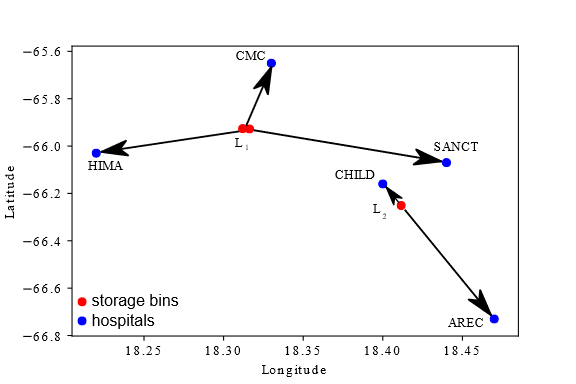
\includegraphics[width=0.7\linewidth]{../storage_fig2}
	\caption[Fig 1]{A grouping of 5 hospitals to 2 locations, with the locations of the storage bins determined by the location of the hospitals and their medical package demands. L1 and L2 represent the storage locations and the blue dots represent the specific hospitals given by their 3-5 letter abbreviation.}
	\label{Fig 1}
	\end{figure}
	


\subsection{Cost Function}
Our cost function is described by the following formula, evaluating for a via flight plan and drone configuration.
\[
C = \alpha \frac{P}{\sum{t}} - \beta \frac{S}{100000}
\]
Where $P$ represents the total medpacks delivered, $\sum{t}$ is an estimate of the time for all the flights to occur, and $S$ represents the space left after packing all the drones (computed via the packing algorithm). Also, $C$ is our cost function output, the cost. The factor of $100000$ dividing $S$ is there to adjust the units of $S$ (it being on the order of $10^5$ while $\frac{P}{\sum{t}}$ is on the order of $10^0$) The time estimates are computed via the basic kinematic equation assuming constant speed, $\sum{t}=\sum{\frac{d}{v_d}}$ summed over all drone flights in the given plan. Here $d$ is distance traveled in a specified flight and $v_d$ is the max speed of the drone flying. This estimate of the time taken for a flight is assuming the drone is flying at max speed the whole way, and assuming equality of the time taken to fly to the hospital, and the time to fly back. The assumption of perfectly sequential ordering of the flights allows us to sum the times of individual flights to get the total time.

\section{Results and Analysis}
% TODO: \usepackage{graphicx} required
\begin{figure*}
	\centering
	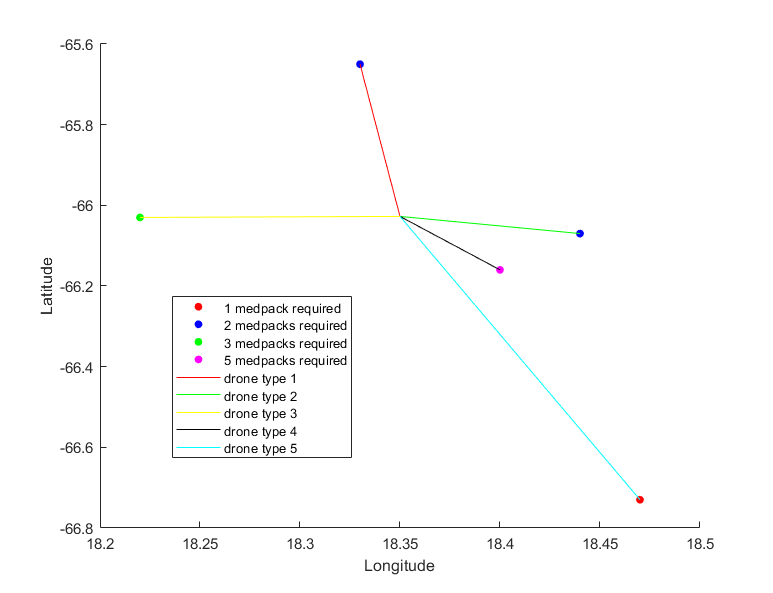
\includegraphics[width=0.7\linewidth]{../example_flight_plan}
	\caption[Fig 1.]{Example optimized flight plan, ran with drone fleet size of 5, starting configuration 1, 5 allowed movements, and $\gamma$ = 2}
	\label{Fig 1.}
\end{figure*}

\subsection{Model output}
Our model output for the customer specifies a drone configuration and a sequence of drone movements: each movement defines an action of a single drone making one flight, and a drone configuration defines how many and of what type the drones used in the system are. In our simplified drone path algorithm, each movement is a straight line path from the starting location to the hospital specified, performed by a specified drone. Our final output is thus a single series of movements and a single configuration, corresponding to the most optimized plan, as determined by our cost function. In figure 1, an example of an optimized model output is shown. 

Although it is not depicted in the figure, a model run will produce multiple viable flight plans, each with their own cost value, enabling the user to select a sub-optimal flight plan later on due to limiting factors not taken into account with our model. Therefore it is necessary to statistically analyze all the cost function outputs for a given model run near the minimum (representing the most optimal flight plan). This analysis was done for studies of parameter sensitivity as well as for directly comparing model outputs.

\subsection{Parameter sensitivity}
The outputs of the cost function were analyzed after varying different parameters to find reasonable values for further analysis. The metric used for comparing the effectiveness of our model outputs is a measure of how many viable flight paths are produced with a cost function value near the minimum. The parameters we varied were the different valid storage bin configurations, the number of allowed movements in a flight plan, and the number of drones in a fleet.

We looked at the outputs of our storage location sub-model for 15 possible configurations of storage bin locations. We limited configurations to two storage bins which we identified as the minimum number needed to understand the effects of having multiple storage bins and the effect that changing those configurations would have on the model output. The results of this study are shown in figure 3.

% TODO: \usepackage{graphicx} required
\begin{figure}
	\centering
	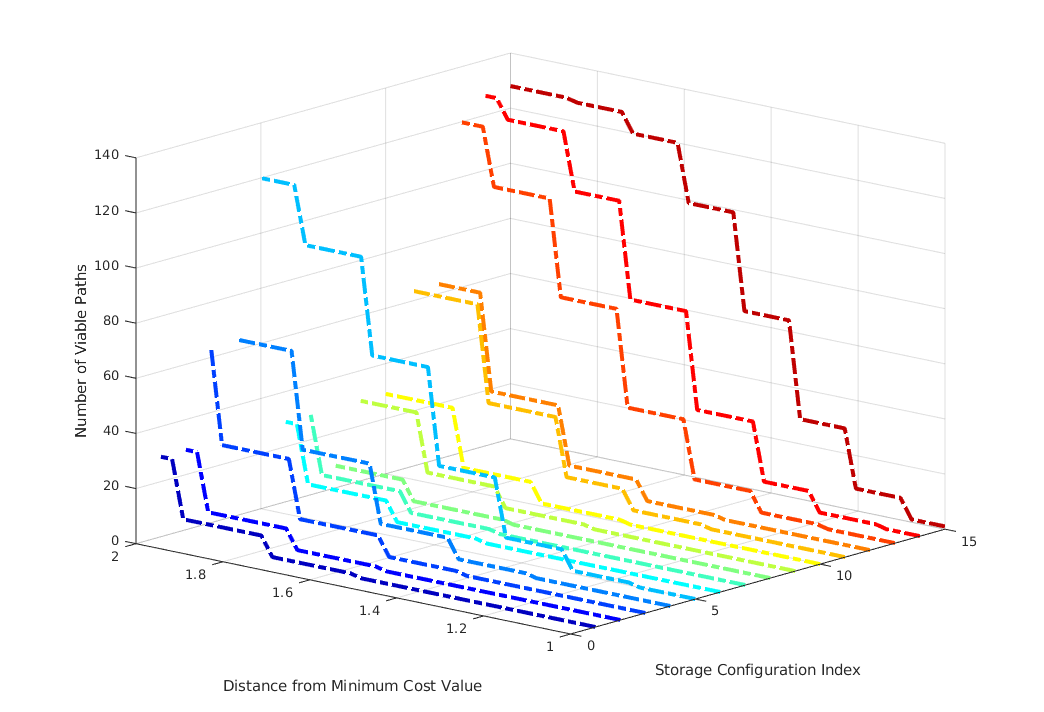
\includegraphics[width=1.1\linewidth]{../cost_output_per_storage}
	\caption[Fig 2]{Model sensitivity to storage container configuration. The different storage configuration indices each correspond to storage locations for drones as outputted by our storage location sub-model. Distance from the minimum was found for each of the several thousand viable flight plans for a certain storage configuration and the number that are within a certain value is reported in each line. Model ran with $gamma=2$ and 7 allowed movements.}
	\label{Fig 3}
\end{figure}
From the figure we see that configurations 15,14,13 and 5 had considerably high numbers of paths being close to optimal. Also, in the outputs for these storage configurations, we see that configurations 5,13,14, and 15 have the 4 lowest minimum costs of all configurations with 15 having the overall minimum. Based on this evidence, it is reasonable to select configuration 15 as the most optimized configuration with 14,5, and 13 also being acceptable.

The number of allowed movements in the flight plan was limited by our hospital requirements. For example, the sum of all required medipacks for a day was 13, so no configuration of only drone B (which can hold only 1 medipack) can have less than 13 movements. Thus, because our max drone capacity was 2 medipacks, our minimum number of allowed movements in a flight plan was 7. Our model did not consider the interaction between the number of allowed movements and the number of drones in the fleet due to our assumption that every drone can make as many or as little trips as possible in a day. There may be an additional interaction between these quantities in terms of the optimized flight plan but our parameter sensitivity was limited to studying sensitivity of individual parameters and not their interactions.

We cannot investigate the outputs of infinitely many allowed movements due to fundamental limitations of our models implementation. But this is a realistic view of the problem because in a single day, you cannot have infinitely many drone movements without infinitely many drones. Our selected parameter range and outputs are shown in figure 4.
% TODO: \usepackage{graphicx} required
\begin{figure}
	\centering
	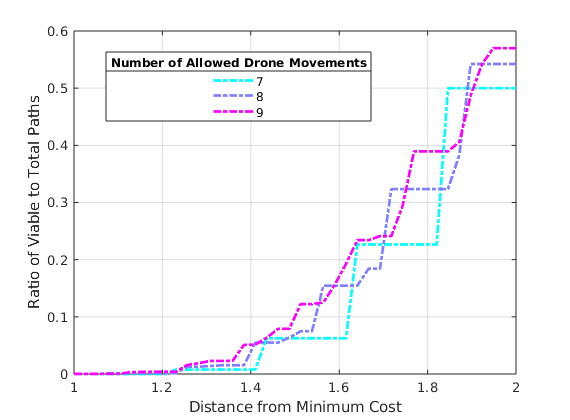
\includegraphics[width=0.9\linewidth]{../cobt2d}
	\caption[Fig 3]{Number of viable flight plans with a cost value close the the minimum (optimized) value. Each color is a different model run varying the number of allowed drone movements. The number of flight plans with a cost cost to the minimum was normalized by total number of viable flight plans given by the run thus the y-axis is a ratio of how many of the total flgiht paths are within that range.}
	\label{Fig 4}
\end{figure}

The curves depicted show no general deviation from their common shape and all rise to roughly the same maximum (between 0.5 and 0.6). However, in looking at the minimum value outputted by the cost function for each of the number of allowed trips, the values get continually lower as the number of allowed trips increases (min of 2.6975 for 7 allowed trips, min of 2.3951 for 8 allowed trips and min of 2.2015 for 9 allowed trips). Because our cost function equally values number of medipacks delivered and the estimated time total for that delivery, these results would suggest that increasing the number of allowed movements increases the number of delivered medipacks faster than it increases the amount of time to deliver these medipacks. However, further investigation may well reveal that below a certain number of allowed movements, the most optimized flight plan is not further improved. 



\subsection{Limitations/ Further Work}
Our cost function is limited given that it favors solutions with fewer drones even in instances when the combined effort of many drones may be more effective than the combined effort of fewer drones. This arises from our assumption of sequential drone paths. A fleet of many drones may be monetarily expensive, but it would allow more time-efficient concurrent delivery. This limitation would be further amplified in larger-scale drone fleet models for which  more complex metrics for medipack delivery efficiency is recommended.

Furthermore, our cost function did not take into account mapping of disaster terrain. This can be reconciled by adjusting our model output after it has been optimized to the current cost function to add curvature that will increase its surveillance coverage of focus areas of land. A metric representing how far it may deviate from the initial straight line path can be applied to the adjusted output to reach a single solution. However, the main limitation of performing this adjustment after the main optimization is that adding this curvature will increase $\sum{t}$ as defined in the cost function and may increase $sum{t}$ unevenly across different viable flight paths. This could lead to a different optimized flight plan after the curvature would have been added. Thus, by adding the curvature after optimized by our cost function we lose the guarantee that our output is the most optimized under our cost function.

Our assumption of perfectly flat 2D terrain without any need to alter the drone path due to obstructions causes us to lose the fundamental aspect of navigation in our drones. A real scenario in which the conditions that the drones must navigate through after a natural disaster are impossible to predict would warrant a stochastic method of modeling terrain obstructions and finding alternate routes. These methods would also be an effective measure of the DroneGo system's ability to operate successfully in any requested environment. How the implementation of a stochastic terrain model might alter the optimized outputs of the model would be an interesting investigation. 

\section{Conclusion}
Based on our model, we recommend that HELP, Inc. groups the hospitals so that the Caribbean Medical Center and Hospital HIMA are serviced by one storage bin located at longitude 18.2640 and latitude -65.878, with and Hospital Pavia Santurce, Puerto Rico Children's Hospital, and Hospital Pavia Arecibo serviced by two storage bins located at longitude 18.4187 and latitude-66.2087 (configuration 15). We also recommend limiting the number of drones used as this will increase space in the in the storage bins allocated to the medical packages, even though it decreases time efficiency of medical package delivery. With this in mind, we recommend selecting drones with a larger drone cargo bay type. According to this model, this will yield the best possible setup for storage and delivery of medical packages in the face of a disaster.


\bibliographystyle{apalike}
\bibliography{asme2ej2.bib}

\end{document}
